
\سؤال{}

\textbf{شرکت‌ها و به‌ویژه شرکت‌های نرم‌افزاری هم مانند انسان‌ها مراحل رشد و شکوفایی دارند. برای بررسی این بلوغ از روش‌هایی مانند \lr{CBA-IPI} که در فصل سوم کتاب مطرح شده، استفاده می‌شود. لطفا با انجام تحقیق کوچکی مراحل مختلف بلوغ سازمان‌ها را در این روش به اختصار مشخص کنید.}


سطح بلوغ یک تکامل خوش‌تعریف\footnote{well-defined} جهشی رو به جلو برای دست‌یابی به یک فرآیند نرم‌افزاری بالغ است. هر سطح بلوغ یک لایه‌ای را در پایه برای بهبود مداوم فرآیند فراهم می‌کند. 
\begin{figure}[!h]
	\begin{center}
		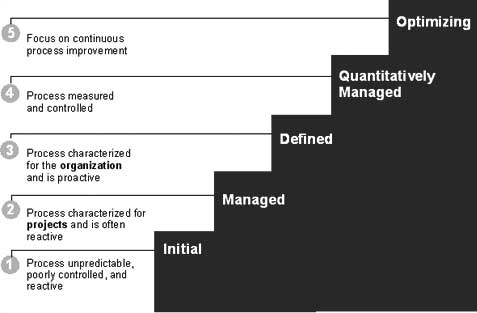
\includegraphics[scale=0.7]{./3.jpg}
	\end{center}
	\caption{مراحل بلوغ در سازمان‌ها}
\end{figure}

در مدل \lr{CMMI} \footnote{Capability Maturity Model Integration} از پنج سطح بلوغ تشکیل شده است:
\begin{enumerate}
	\item سطح اولیه\footnote{Initial}
	\item سطح مدیریت شده
	\item سطح تعریف شده
	\item سطح مدیریت شده از نظر کمّی\footnote{\lr{Quantitatively Managed}}

	\item سطح بهینه‌سازی
	
\end{enumerate}

حال هر سطح از سطوح بالا را به‌طور دقیق‌تر بررسی می‌کنیم:

\begin{itemize}
	\item 
	\textbf{سطح اولیه}
	
	در این سطح فرآیند‌ها معمولا نامشخص هستند. سازمان معمولا محیط پایداری را فراهم نمی‌کند و موفقیت در این سازمان‌ها ببیش‌تر ستگی به رقابت افراد و اعضای و نه استفاده از فرآیند‌های اثبات شده دارد. در این مرحله بعضی اوقات محصول یا سرویسی تولید می‌شود اما  قیمت تمام‌شده‌ی آن‌ها معمولا بالاتر از بودجه‌ی اختصاص داده شده است.
	\item 
	\textbf{سطح مدیریت شده}
	
	در این سطح سازمان به همه‌ی اهداف کلی و خاص رسیده است. به بیان دیگر، پروژه‌های سازمان تضمین کرده‌اند که نیازمندی‌ها مدیریت می‌شوند و هم‌چنین فرآیندها نیز برنامه‌ریزی، انجام، اندازه‌گیری و کنترل می‌شوند.
	
	در این مرحله تعهدات بین سهام‌داران ایجاد شده و در صورت نیاز مورد بازبینی و تجدید نظر قرار می‌گیرد.
	
	\item
	\textbf{سطح تعریف شده}
	
	در این سطح فرآیندها به خوبی مشخص و درک شده و در قالب استاندارد‌ها، رویه‌ها\footnote{procedure}، ابزارها و روش‌ها بیان می‌شوند.
	تفاوت اصلی و مهم بین سطح شماره‌ی «۳» و «۲» در محدوده استانداردها، توضیحات فرآیندها و رویه‌ها می‌باشد. در سطح «۲» استانداردها، توضیحات فرآیند و رویه‌ها ممکن است در هر نمونه خاص از فرآیند (مانند یک پروژه خاص) کاملا متفاوت باشند اما در مورد «۳» این تفاوت وجود ندارد و سازمان یک‌پارچه است.
	
	\item 
	\textbf{سطح مدیریت شده از نظر کمّی}
	
	در این سطح فرآیندهای فرعی که به‌طور قابل توجهی در عملکرد \footnote{performance}کلی فرآیند تاثیرگذارند، انتخاب می‌شوند. این فرآیندها با استفاده از روش‌های آماری و دیگر تکنیک‌های اندازه‌گیری کمّی کنترل می‌شوند. اهداف کمّی به عنوان معیاری برای مدیریت فرآیند‌ها ایجاد می‌شوند. این اهداف براساس نیازهای مشتری، کاربران نهایی\footnote{end users}، سازمان‌ها و مجریان فرآیند هستند.
	
	تفاوت اصلی این سطح با سطح شماره‌ی «۳» «قابلیت پیش‌بینی عمل‌کرد فرآیندها» است.
	
	\item 
	\textbf{بهینه‌سازی}
	
	در این سطح فرآیند‌ها به‌طور مداوم بر اساس درک کمّی از دلایل مشترک تغییر ذاتی فرآیند‌ها بهبود می‌یابند و بیش‌تر تمرکز آن بر روی پیشرفت ادامه‌پذیر عمل‌کرد فرآیند از طریق کارهای تکراری-افزایشی\footnote{iterative and incremental} است.
	
	این سطح در مقایسه با سطح «۴» در این مورد تفاوت دارند که در آن مشکلی  برای کافی بودن عوامل برای دست‌یابی به نتایج  اهداف وجود ندارد
\end{itemize}

\textbf{نکته} هر کدام از سطوح گفته شده ضروری هستند و نباید از آن‌ها پرش کرد.\footnote{skip} در صورت پرش کردن، هر چه سطح بالاتر باشد، احتمال رسیدن به موفقیت کم‌تر می‌شود.